\documentclass[ngerman]{scrbook}
\usepackage{color}
\usepackage{xspace}
\usepackage{enumitem}
\usepackage{listings, tabularx, graphicx, subcaption}
\usepackage[german]{babel}

\usepackage{hyperref}
\usepackage{cleveref}
\newcommand{\gamefile}[1]{\textit{\textcolor{blue}{#1}}\xspace}
\newcommand{\game}{\gamefile{game.xml}}
\newcommand{\gameinstance}{\gamefile{game\_instance.xml}}

\newcommand{\card}{\textcolor{red}{card}\xspace}
\newcommand{\gamefigure}{\textcolor{red}{figure}\xspace}
\newcommand{\dice}{\textcolor{red}{dice}\xspace}
\newcommand{\book}{\textcolor{red}{book}\xspace}
\newcommand{\boxtype}{\textcolor{red}{box}\xspace}
\newcommand{\xmlattribute}[1]{\textcolor{green}{#1}}


\definecolor{maroon}{rgb}{0.5,0,0}
\definecolor{darkgreen}{rgb}{0,0.5,0}
\lstdefinelanguage{XML}
{
	basicstyle=\ttfamily,
	morestring=[s]{"}{"},
	morecomment=[s]{?}{?},
	morecomment=[s]{!--}{--},
	commentstyle=\color{darkgreen},
	moredelim=[s][\color{black}]{>}{<},
	moredelim=[s][\color{red}]{\ }{=},
	stringstyle=\color{blue},
	identifierstyle=\color{maroon}
}


\title{Boardgame Simulator Anleitung}
\begin{document}
	\maketitle
	\tableofcontents
	\chapter{Kurzanleitung}
	
	Dies ist eine kurze Schritt-für-Schritt Anleitung um einen Server zu starten und vorhandene Spiele zu laden. Möchte man nur zu einem vorhandenen Server verbinden und ein neues Spiel laden, können die Punkte \ref{item:DynDns}-\ref{item:StartServer} übersprungen werden. Wie man neue Spiele erstellt, wird in \Cref{chap:createGames} erklärt.
	
	\begin{enumerate}[label=\arabic*)]
		\item \textbf{Java installieren:} Für das Programm wird Java benötigt. Java kann unter folgendem Link \href{https://www.java.com/de/download/}{https://www.java.com/de/download/} heruntergeladen werden und installiert werden.
		
		\item \label{item:DynDns} \textbf{DynDNS Adresse erstellen und mit Router verbinden:} Mithilfe einer festen Adresse Adresse kann Verbindung zum Spiel vereinfacht werden. Solche Adressen können zum Beispiel auf der Seite \href{https://www.noip.com}{https://www.noip.com} kostenlos erstellt werden und sehen wie folgt aus \textit{meinspieleserver.ddns.net}. Diese Adresse muss im jeweiligen Router hinterlegt werden. Je nach Routermodell kann das etwas unterschiedlich funktionieren!
		\begin{enumerate}
			\item \textbf{Fritz-Box:} \href{https://avm.de/service/fritzbox/fritzbox-7590/wissensdatenbank/publication/show/30_Dynamic-DNS-in-FRITZ-Box-einrichten/}{Link zum Tutorial} 
			\item \textbf{Telekom:} \href{https://www.netzwelt.de/news/95517-anleitung-dyndns-speedport-routern-einrichten.html}{Link zum Tutorial}
		\end{enumerate}
		
		\item \textbf{Port freischalten:} Auf dem Router muss nun noch der Port freigeschaltet werden über den der Server läuft, damit die Mitspieler von außerhalb des lokalen Netzes auf den Server zugreifen können.
		
		\item \label{item:StartServer} \textbf{Server starten:} 
			Zuerst zum Programmpfad navigieren  in dem die Datei SimpleBoardGameSimulator.jar liegt.
		\begin{enumerate}
			\item \textbf{Windows:} Die Datei StartServer.bat, die im selben Verzeichnis liegt mit einem Texteditor öffnen und $<$port$>$ durch den freigeschalteten Port ersetzen.
			\item \textbf{Linux:} Im Terminal den Befehl 
			$$\mbox{java -jar SimpleBoardGameSimulator.jar --server $<$port$>$}$$ ausführen. $<$port$>$ muss durch den freigeschalteten Port ersetzt werden!
		\end{enumerate}
		
		\item \label{item:StartGame} \textbf{Programm starten:} Das Programm SimpleBoardGameSimulator.jar ausführen. Nun sollte sich folgendes Fenster öffnen:
		\begin{figure}[!h]
			\centering
			     \begin{subfigure}[b]{0.45\textwidth}
				\centering
				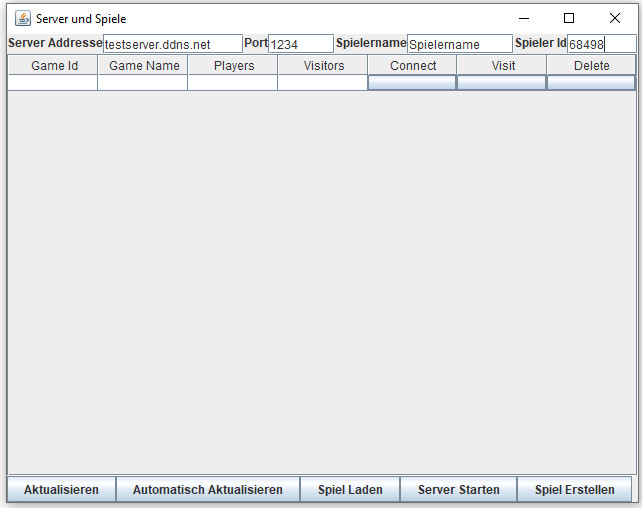
\includegraphics[width=\textwidth]{ServerLobbyWindow.jpg}
				\caption{Startfenster des Spiels}
				\label{fig:Start}
			\end{subfigure}
			\hfill
			\begin{subfigure}[b]{0.45\textwidth}
				\centering
				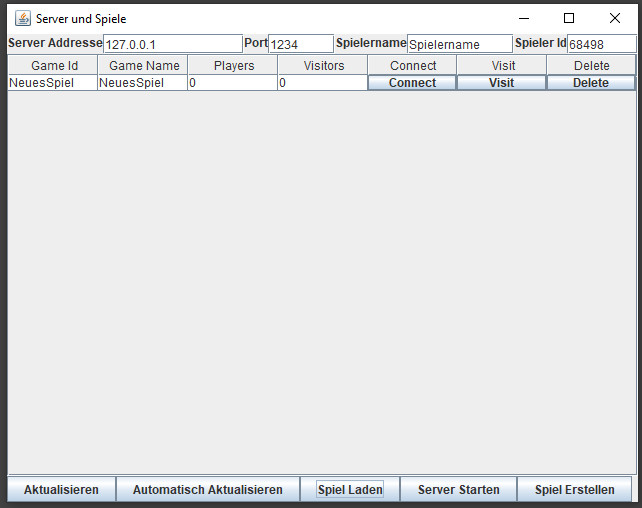
\includegraphics[width=\textwidth]{ServerLobbyWindowStartedGame.jpg}
				\caption{Startfenster mit geladenem Spiel}
				\label{fig:StartLoaded}
			\end{subfigure}
			\caption{Startfenster des Spiels}
		\end{figure}
	
		Als Serveradresse muss nun die Adresse des Servers eingegeben werden (entweder die oben erstellte Adresse oder die Adresse eines vorhandenen Servers mit dem man verbinden möchte). Als Port muss der zuvor freigeschaltete Port eingegeben werden oder der Port des vorhandenen Servers mit dem man verbinden möchte. Jeder Spieler kann sich einen Namen geben und sollte eine eindeutige Spieler Id wählen. Falls schon ein Spiel auf dem Server läuft kann ``Aktualisieren'' gedrückt werden um das Spiel anzuzeigen. Dann erscheint wie im Bild rechts das laufende Spiel und die Spieler können mit dem ``Connect'' Button verbinden.
		
		\item \textbf{Spiel laden:} Wenn sich das Programmfenster geöffnet hat kann über den Button ``Spiel Laden'' ein neues Spiel, das man schon erstellt hat, geladen werden. Dazu navigiert man im Fenster, das sich öffnet zum Spiel (z.B. Spiel.zip) und klickt auf ``Öffnen''. Das Spiel sollte nun für alle Spieler, die die richtige Adresse und den richtigen Port angegeben haben erscheinen, wenn sie auf ``Aktualisieren'' klicken. Klicken auf ``Connect'' lässt die Spieler mit dem Spiel verbinden.
	\end{enumerate}
	
	
	\chapter{Spiel erstellen}\label{chap:createGames}
	In diesem Abschnitt wird beschrieben, wie ein neues Spiel für den Brettspielsimulator erzeugt werden kann. 
	
	Jedes Spiel besteht aus Spielobjekten (Bildern im jpg oder png Format) und den XML-Dateien \game und \gameinstance. Spielobjekte können drei verschiedene Typen haben \card, \gamefigure und \dice.
	\section{Die Datei \game}
	In der \game werden die Spielobjekte definiert. Das Grundgerüst der Datei sieht wie folgt aus. 
	
	\lstset{language=XML}
	\begin{lstlisting}
	<?xml version="1.0" encoding="UTF-8" standalone="yes"?>
	<xml>
	<background>hintergrund.jpg</background>
	</xml>
	\end{lstlisting}
	
	Das Bild mit dem Namen \textit{hintergrund.jpg} wird zum Hintergrundbild des Spiels.

	Zusätzlich können beliebige Spielobjekte durch den Tag \lstset{language=XML}
	\begin{lstlisting}
	<object type="card"></object>
	\end{lstlisting}  mit den unten genannten Typen definiert werden (in diesem Fall vom Typ \card). Welche Attribute die verschiedenen Spielobjekte haben können wird in den entsprechenden Abschnitten erläutert.

	\section{Die Datei \gameinstance}
	In der \gameinstance wird eine Instanz des Spiels definiert, z.B. ob es einen Tisch geben soll oder nicht und an welcher Stelle die Objekte im Spiel zu Beginn liegen.
	
	\lstset{language=XML}
	\begin{lstlisting}	
	<?xml version="1.0" encoding="UTF-8" standalone="yes"?>
	<xml>
	<settings>
		<name>Brettspiel</name>
		<table color="#d2a56d" put_down_area="true"
		table_radius="500">true</table>
	</settings>
	<object unique_name="object1" x="0" y="0" r="0"/>
	</xml>
	\end{lstlisting}
	
	Das Beispiel definiert ein Spiel mit dem Namen \textit{Brettspiel}, das ein Tisch mit Radius $500$, der Farbe $\#d2a56d$, und einem Ablagebereich in der Mitte des Tisches hat. Das Spiel hat außerdem ein Objekt mit dem Namen \textit{objekt1}, welches in \game definiert wurde und an Position $0, 0$ und mit Anfangsrotation $0$ gezeichnet wird.
	
	Unter dem Tag \textit{settings} können alle wichtigen Spieleigenschaften definiert werden. Unter dem Tag \textit{object} werden die Objekte mit Positionen, Rotationen usw. definiert.
	
	\begin{table}[!h]
		\centering
		\renewcommand{\arraystretch}{1.5}
		\begin{tabularx}{\textwidth}{c|X|c|X}
			Tagname & Attribute & Werte & Erklärung\\\hline
			
			name & -- & String & Name des Spiels\\
			table & \xmlattribute{color}, \xmlattribute{put\_down\_area}, \xmlattribute{table\_radius} & true/false & Anzeige des Tisches auf dem Spielfeld, falls False wird der Tisch nicht angezeigt, \xmlattribute{color} definiert die Farbe des Tisches, \xmlattribute{put\_down\_area} ist ein boolsches Attribut und gibt an, ob ein Ablagebereich in der Mitte des Tisches erscheinen soll, \xmlattribute{table\_radius} gibt den Radius des Tisches an.\\
			private\_area & -- & true/false & gibt an, ob der Handkartenbereich zum Spielstart eingeblendet sein soll\\
			seats & -- & $<$seat color="\#0000ff"/$>$ & Feste Liste von farbigen Stühlen um den Tisch\\
			debug\_mode & -- & true/false & Falls true, werden zusätzliche Informationen angezeigt, die hilfreich beim debuggen sind\\
		\end{tabularx}
	\caption{Mögliche Spiel Settings}
	\end{table}
	\section{Spielobjekttypen}
	
	Die Spielobjekte werden in der \game definiert. Einzelne Instanzen von Spielobjekten werden in der \gameinstance definiert und mit einem eindeutigen Namen mit den Objekten aus der \game verknüpft. Spielobjekte werden durch den Tag \textit{object} markiert. Alle Spielobjekte haben die folgenden Attribute.
	
	\begin{table}[!h]
		\renewcommand{\arraystretch}{1.5}
		\begin{tabularx}{\textwidth}{XX}
			Attribute & Erklärung\\\hline
			type & Typ des Spielobjekts\\
			unique\_name & Eindeutiger Name des Objekts\\
			width & Breite des Objekts\\
			height & Höhe des Objekts\\
		\end{tabularx}
	\end{table}

	Weitere Attribute für \card, \gamefigure, \dice Objekte können in den jeweiligen Abschnitten gefunden werden.

	Instanzen von Spielobjekten können in der \gameinstance mit folgenden Attributen definiert werden:
	
	\begin{table}[!h]
		\renewcommand{\arraystretch}{1.5}		\begin{tabularx}{\textwidth}{XXX}
			Attribute & Erklärung\\\hline
			unique\_name & eindeutiger Name aus der \game\\
			x & x Position zu Spielbeginn\\
			y & y Position zu Spielbeginn\\
			r & Rotation\\
			s & Skalierung\\
			number & Anzahl der Objekte des Typs\\
			value & Wert des Objekts\\
			sortValue & Sortierwert des Objekts, die Handkarten werden anhand dieses Werts sortiert\\
			number & Anzahl der Objekte des Typs\\
			boxId & Id der Box in der das Objekt zum Spielbeginn liegen soll\\
			inBox & true/false, falls true liegt das Objekt in der Box mit boxId sonst nicht\\
			is\_fixed & true/false, falls true kann Objekt im Spiel nicht bewegt werden\\
		\end{tabularx}
	\end{table}

	Beispieldefinition von Instanzen des Objekts mit dem Namen \textit{objekt1} in der \gameinstance:
	
	\lstset{language=XML}
	\begin{lstlisting}
	<object unique_name="objekt1" x="0" y="0" r="0" s="1" 
	 number="3" boxId="1" is_fixed="false"/>
	\end{lstlisting}
	
	In diesem Beispiel werden $3$ Instanzen vom Objekt mit dem Namen \textit{objekt1} an der Position $0,0$ mit der Rotation $0$ und ohne Skalierung erzeugt.

	
	\subsection{Der Typ \card}
	Objekte vom Typ \card sind Spielkarten. Sie können z.B. gestapelt und gemischt werden und haben eine Vorder-und Rückseite.
	Beispiel eines \card Objekts mit Vorderseite \textit{front.jpg}, Rückseite \textit{back.jpg}, dem Wert $10$ hat und in $45$ Grad Schritten gedreht werden kann und zur Kartengruppe \textit{Spielkarte} gehört:
	
	\lstset{language=XML}
	\begin{lstlisting}
	<object type="card" unique_name="card1" value="10"
	 rotation_step="45" front="front.jpg" back="back.jpg">
	 <group>Spielkarte</group>
	</object>
	\end{lstlisting}
	
	\begin{table}[!h]
		\renewcommand{\arraystretch}{1.5}		\begin{tabularx}{\textwidth}{XXX}
			Attribute & Optional & Erklärung\\\hline
			front & Nein & Dateiname der Vorderseite (jpg, png)\\
			back & Nein & Dateiname der Rückseite (jpg, png)\\
			value & Ja & Wert der Karte\\
			rotation\_step & Ja & Mögliche Rotationen der Karte\\
		\end{tabularx}
	\end{table}

	Objekte vom Typ \card können als Wert eine Gruppe erhalten über die sie eindeutig identifizierbar und sammelbar sind.

	\lstset{language=XML}
	\begin{lstlisting}	
	<group>Spielkarte</group>
	\end{lstlisting}

	\subsection{Der Typ \gamefigure}
	Objekte vom Typ \gamefigure sind Spielfiguren. Sie können z.B. stehen oder liegen und auf Karten gestellt werden.

	Beispiel eines \gamefigure Objekts:
	
	\lstset{language=XML}
	\begin{lstlisting}	
	<object type="figure" unique_name="objekt1"
	 standing="standing.jpg" width="100" 
	 height="100"/>
	\end{lstlisting}
	

	\begin{table}[!h]
		\renewcommand{\arraystretch}{1.5}
		\begin{tabularx}{\textwidth}{XXX}
			Attribute & Optional & Erklärung\\\hline
			standing & Nein & Bild für die stehende Spielfigur (jpg, png)
		\end{tabularx}
	\end{table}


	\subsection{Der Typ \dice}
	Objekte vom Typ \dice sind Würfel. Sie haben mehrere Seiten und können gewürfelt werden.

	Beispiel eines \dice Objekts mit sechs Seiten:
	
	\lstset{language=XML}
	\begin{lstlisting}	
	<object type="dice" unique_name="dice1" width="30" height="30">
		<side value="1">side1.jpg</side>
		<side value="2">side2.jpg</side>
		<side value="3">side3.jpg</side>
		<side value="4">side4.jpg</side>
		<side value="5">side5.jpg</side>
		<side value="6">side6.jpg</side>
	</object>
	\end{lstlisting}
	
	Objekte vom Typ \dice haben als Werte Seitenobjekte mit Tag \textit{side}, mit einem Attribut \xmlattribute{value} und als Wert das Bild der Seite.

	\subsection{Der Typ \book}
	Objekte vom Typ \book können wie Bücher verwendet werden. Sie haben mehrere Seiten und können vor-und zurück geblättert werden.
	
	Beispiel eines \book Objekts mit sechs Seiten:
	
	\lstset{language=XML}
	\begin{lstlisting}	
	<object type="book" unique_name="book1" width="30" height="30">
		<side value="1">side1.jpg</side>
		<side value="2">side2.jpg</side>
		<side value="3">side3.jpg</side>
		<side value="4">side4.jpg</side>
		<side value="5">side5.jpg</side>
		<side value="6">side6.jpg</side>
	</object>
	\end{lstlisting}
	
	Objekte vom Typ \book haben als Werte Seitenobjekte mit Tag \textit{side}, mit einem Attribut \xmlattribute{value} und als Wert das Bild der Seite.
	
		\subsection{Der Typ \boxtype}
	Objekte vom Typ \boxtype können wie eine Spielbox verwendet werden. Objekte mit dem Attribut \xmlattribute{boxId}$="x"$ befinden sich zum Spielstart in der Box mit \xmlattribute{boxId}$="x"$
	
	Beispiel eines \boxtype Objekts:
	
	\lstset{language=XML}
	\begin{lstlisting}	
		<object type="box" unique_name="game_box" width="30" height="30" front="front.jpg" back="back.jpg"></object>
	\end{lstlisting}
	
	Objekte vom Typ \book haben als Werte Seitenobjekte mit Tag \textit{side}, mit einem Attribut \xmlattribute{value} und als Wert das Bild der Seite.


	\chapter{Spielsteuerung}
\end{document}